
\section{Premières mesures du temps d'exécution}

\subsection{Paramètres utilisés dans toute cette section}
% Indiquez ici les valeurs de $m$ et $k$ avec lesquelles vous avez travaillé pour cette section. Indiquez également le ou les fichiers d'entrée utilisé(s) et la ou les valeur(s) de $n$ correspondantes. Indiquez également votre environnement de travail : système d'exploitation, compilateur (version), options de compilation, processeur, mémoire vive, etc. 

% ** PARAMETRES UTILISES
% ** FICHIER(S)
% [DONE] ** ENVIRONNEMENT DE TRAVAIL

\subsubsection{Paramètres}

Étant donné que les tests n'ont pas été réalisés avec les mêmes paramètres à chaque fois, ceux-ci sont indiqués lorsqu'ils sont utilisés.


\subsubsection{Environnement de travail}
\begin{table}[h!]
	\centering
	\caption{Informations sur la machine utilisée.}
	\label{tab:environnementTravail}
	\begin{tabular}{c|c}
		\toprule
		OS & Microsoft Windows 10 Professionnel 10.0.10240\\
		Processeur & Intel(R) Core(TM) i7-4702MQ CPU @ 2.20GHz 4 coeurs 8 processeurs logiques\\
		Memoire & 7.66GB DDR3\\
		Disque & 1TB HDD Toshiba MQ01ABD100\\
		Compilateur & gcc 4.8.1 (Windows 10)\\
		\bottomrule
	\end{tabular}
\end{table}

% Pour chacune des sous-sections suivantes, indiquez le nombre de runs effectués pour soutenir vos résultats.

\subsection{Mise en évidence de la stochasticité de l'algorithme}
% Montrez la variabilité obtenue dans les temps d'exécution en incluant un histogramme du temps CPU dans votre rapport (Figure \ref{fig:histo-variabilite}). Quantifiez cette variabilité en indiquant l'écart-type de ce temps d'exécution (sans oublier de préciser le nombre de runs sur lequel cet écart-type a été calculé). 

% \begin{figure}[htbp]
% 	\begin{center}
% 		% remplacez par votre figure 
% 		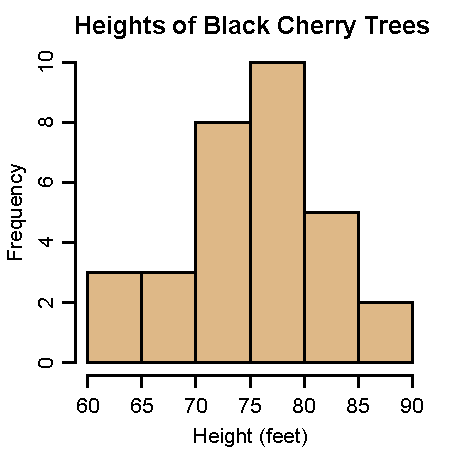
\includegraphics[width=6cm]{Black_cherry_tree_histogram.pdf}
% 		\caption{Black cherry tree histogram. Source: Wikimedia Commons.}
% 		\label{fig:histo-variabilite}
% 	\end{center}
% \end{figure}



% ** MONTRER VARIABILITE -> Histogramme

\begin{figure}[htbp]
	\begin{center}
		\includegraphics[width=6cm,height=6cm]{diagrams/time_m_10000_k_2.pdf}
		\caption{.}
		\label{fig:timeM10000K2}
	\end{center}
\end{figure}
Nous pouvons voir sur la figure \ref{fig:timeM10000K2} différents paliers représentant les différents fichiers d'entrée.
Chaque temps mesuré d'un palier (donc d'un fichier) est une execution identique les unes par rapport aux autres.
Nous voyons donc qu'au sein d'un même palier, les temps varient, représentant la stochasticité de l'algorithme.

\begin{figure}[htbp]
	\begin{center}
		\includegraphics[width=6cm,height=6cm]{diagrams/time_m_100000_k_2.pdf}
		\caption{.}
		\label{fig:timeM100000K2}
	\end{center}
\end{figure}
Sur la figure \ref{fig:timeM100000K2}, nous pouvons voir une stochasticité plus importante, surement dû à une valeur de m 10 fois plus grande.

\begin{figure}[htbp]
	\begin{center}
		\includegraphics[width=6cm,height=6cm]{diagrams/time_m_100000_k_2_n_39213.pdf}
		\caption{.}
		\label{fig:timeM100000K2n39213}
	\end{center}
\end{figure}
La figure \ref{fig:timeM100000K2n39213} montre la stochasticité de l'algorithme sur un seul palier. C'est à dire que tous les points représentent le temps d'execution avec des paramètres identiques.

% ** ECART-TYPE


\begin{table}[h!]
	\centering
	\caption{Valeurs de $n$ choisies.}
	\label{tab:ecartTypesTemps}
	\begin{tabular}{ccc|c}
		\toprule
		m & k & n & Ecart-type\\
		\midrule
		100000 & 2 & 39213 & 24.35136 ms\\
		100000 & 7 & 39213 & 31.43317 ms\\
		100000 & * & 39213 & 29.36821 ms\\
		\bottomrule
	\end{tabular}
\end{table}


% ** NB RUNS
Ces tests ont été réalisés en 10 runs.



% Puis décrivez la manipulation que vous avez effectuée pour montrer qu'une grande part de cette variabilité provient de la stochasticité de l'algorithme. 

Nous avons appliqué à $srand$ une valeur fixe (ici, 0), ainsi, à chaque execution de mêmes paramètres, les résultats seront très proches les uns des autres. Cela peut être clairement vu sur la figure \ref{fig:timeStochasticite}, avec, en noir, 100 exécutions avec une graine qui change, et en rouge, 100 exécutions avec une graine constante.

\begin{figure}[htbp]
	\begin{center}
		\includegraphics[width=6cm,height=6cm]{diagrams/time_serial_paral.pdf}
		\caption{.}
		\label{fig:timeStochasticite}
	\end{center}
\end{figure}

\subsection{Influence de la charge système}
% En vous appuyant sur le cours, expliquez pourquoi le temps CPU, bien que fait pour être le plus indépendant possible de la charge système, peut tout de même être influencé par la charge système en pratique. Décrivez l'expérience que vous avez effectuée pour tester cet effet et synthétisez-en les résultats, en appuyant vos affirmations sur des chiffres. 

% ** PK TMPS CPU INFLUENCé PAR LA CHARGE SYSTEME?
Le temps CPU est influencé par la charge système car si celui-ci est très demandé par d'autres processus, alors il y a plus de chance pour que le processeur soit coupé entre deux mesures de temps pour donner la main à un autre processus.

% ** DECRIRE EXPERIENCE
Pour observer ce phenomène, il suffit de lancer les tests en série et des les comparer aux mêmes tests lancés en parallèle.
Etant donné que le système va devoir passer d'un processus à l'autre, nous observerons donc des différences.

% ** DONNER RESULTATS CHIFFRéS
100 tests chacun.

Paramètres : k=3 ; m=100000; fichier=6640.txt

Pour pouvoir observer en grande précision, les tests ont été fait en mesurant non pas le temps, mais un compteur incrémenté par le système (qui représente le temps lorsqu'il est divisé par la fréquence du processeur), ce qui a été fait pour être facilement analysable par des humains.

\begin{table}[h!]
	\centering
	\caption{Résultats.}
	\label{tab:resultatTemps}
	\begin{tabular}{c|cc}
		\toprule
		& Série & Parallèle\\
		\midrule
		Ecart-type & 0.005357606 & 0.02199298\\
		Minimum & 0.004862 & 0.007019\\
		Maximum & 0.031609 & 0.097435\\
		Moyenne & 0.00938539 & 0.0249153\\
		Médiane & 0.0075155 & 0.0155945\\
		\bottomrule
	\end{tabular}
\end{table}

\begin{figure}[htbp]
	\begin{center}
		\includegraphics[width=12cm,height=12cm]{diagrams/time_serial_paral.pdf}
		\caption{.}
		\label{fig:timeSerialParal}
	\end{center}
\end{figure}
En rouge, nous pouvons voir le temps d'exécution en parallèle.
En noir, nous pouvons voir le temps d'exécution en série.
Les lignes représentent les moyennes.


\subsection{Influence des options de compilation}
% Quantifiez le gain de performance obtenu en passant d'une compilation en mode debug à une compilation en mode release (option d'optimisation) : indiquez le pourcentage d'amélioration ainsi que la façon dont vous l'avez calculé (formule, mais aussi nombre de runs, etc).

% ** GAIN PERFORMANCE ENTRE DEBUG ET RELEASE

% Histogramme optimisation
% black = O0
% blue = O1
% orange = O2
% red = O3

\begin{figure}[htbp]
	\begin{center}
		\includegraphics[width=12cm,height=12cm]{diagrams/time_optimisation.pdf}
		\caption{.}
		\label{fig:timeOptimisation}
	\end{center}
\end{figure}

Nous pouvons constater sur la figure \ref{fig:timeOptimisation} que si l'optimisation n'a pas été activée (noir) ou si elle a été activée au niveau 1 (bleu), cela n'implique aucun changement de temps d'exécution. Mais à partir de l'optimisation de niveau 2 (orange), on constate une amélioration. L'optimisation de niveau 3 (rouge) n'implique aucune amélioration par rapport au niveau 2.


% ** % d'amélioration
% ** FORMULE
$moyenne(tempsDebug) = 0.00981731$
$moyenne(tempsRelease) = 0.006638$
$moyenne(tempsRelease) / moyenne(tempsDebug) = 0.6761526$ => Amélioration de 67.61526 \%.

% ** NB RUNS, ...
100 runs pour chaque paramètre d'optimisation.
Paramètres : k=3 ; m=100000; fichier=6640.txt
Optimisations : 0, 1, 2, 3

